
\chapter{Model Checking}


\section{Frame Temporale}

chiamiamo frame temporale un generico frame

$\tau=(T,\,<)$

dove < è una relazione irriflessiva e transitiva.

Posto V una funzione di valutazione, un modello su un frame temporale
è:

$\mu=(\tau,\, V)$

Le logiche basate sui frame temporali si chiamano logiche (modali)
temporali.

Il frame temporale può avere alcune proprietà, infatti si dice:
\begin{itemize}
\item Lineare a destra: $\forall x,y,z((x<y\,\wedge\, x<z)\implies(y<z\,\vee\, z<y\,\vee\, y=z))$ 
\item Lineare a sinistra: $\forall x,y,z((x>y\,\wedge\, x>z)\implies(y>z\,\vee\, z>y\,\vee\, y=z))$ 
\item Ramificato a destra: se non è lineare a destra
\item Ramificato a sinistra: se non è lineare a sinistra
\item Discreto: $\forall x,y(x<y\implies\exists z(x<z\,\wedge\,\neg\exists u(x<u\,\wedge\, u<z)))$
\item Denso: $\forall x,y(x<y\implies\exists z(x<z<y))$
\end{itemize}

\section{Logica LTL}


\subsection{Notazione modena}

La logica LTL ha una notazione più nuova rispetto a quella inizialmente
formulata con gli operatori $\square,\,\diamond,\,\circ$:
\begin{itemize}
\item $\mathcal{G}\equiv[F]$ chiamato ``globally''
\item $\mathcal{F}\equiv<F>$ chiamato ``eventaully''
\item $\mathcal{X}\equiv\circ$ chiamato next
\item $\mathcal{U}$ chiamato until
\item $\mathcal{R}$ chiamato release
\end{itemize}

\subsection{Operatori modali ed espressività della logica}

Dimostriamo Ora alcune proprietà degli operatori di LTL:
\begin{enumerate}
\item $\mathcal{X}$ può essere espresso da $\mathcal{U}$ 
\item $\mathcal{G}$ può essere espresso tramite il solo operatore  $\mathcal{U}$ 
\item $\mathcal{F}$ può essere espresso tramite il solo operatore $\mathcal{U}$ 
\item $\mathcal{X}$ non può essere espresso con $\mathcal{G}$ e $\mathcal{F}$ 
\end{enumerate}
Si dimostra abbastanza facilmente:

1) ricordando che next ha il significato seguente:

$\veraw{\mu}s{\next a}\iff\veraw{\mu}{s+1}a$

consideriamo la seguente formula:

$\veraw{\mu}n{\until{\bot}a}$

è vera se e solo se vale la seguente:

$\exists m>n(\veraw{\mu}ma\,\wedge\,\forall k(n<k<m\implies\veraw{\mu}k{\bot}))$

poichè $\veraw{\mu}k{\bot}$ è falsa in ogni mondo, deve essere falso
l'antecedente dell'implicazione, quindi non deve esistere nessun k
tale che $n<k<m$

Allora avremo che:

$m=n+1$

e quindi

$\veraw{\mu}n{\until{\bot}a}\iff\veraw{\mu}n{\next a}$

2 e 3) Possiamo esprimere l'eventually (e quindi il globally) facilmente
come:

$\eventually a\equiv\until{\top}a$

e quindi:

$\neg\globally{\neg a}\equiv\until{\top}a$

$\globally a\equiv\neg(\until{\top}{\neg a)}$

infatti:

$\veraw{\mu}s{\until{\top}a}\iff\exists t(s<t\,\wedge\,\veraw{\mu}ta\,\wedge\,\forall k(s<k<t\implies\veraw{\mu}k{\top})$

ma poichè $\forall k(s<k<t\implies\veraw{\mu}k{\top})$ è sempre vera,
perchè il conseguente è sempre vero, allora abbiamo:

$\exists t(s<t\,\wedge\,\veraw{\mu}ta)$

che è la definizione di eventually.

4) Supponiamo per assurdo che si possa esprimere l'operatore next
in funzione di globally e eventually.

allora prendiamo il frame:

$N=(\mathbb{N},\,<)$

e usiamo la seguente valutazione:

$V(P)=\{3n\,|\, n\in\mathbb{N}\}$

quindi il modello sarà:

$\mu=(N,\, V)$

allora, per ogni formula ben formata si ha che:

$\veraw{\mu}na\iff\veraw{\mu}{n+3}a$

e

$\veraw{\mu}1a\iff\veraw{\mu}2a$

Per dimostrarlo, uso la bisimulazione:
\begin{itemize}
\item $(\mu,\, n)\leftrightarroweq(\mu,\, n+3)$
\item $(\mu,\,1)\leftrightarroweq(\mu,\,2)$
\end{itemize}
Nel primo caso, costruisco E tale che:

$(n,\, m)\in E\iff m=n+3$

<\textcompwordmark{}<MANCA! non ci ho capito molto, pessimi appunti...>\textcompwordmark{}>


\section{Logiche per il model checking}


\subsection{Logiche per il model checking e semantica}

le principali logiche usate nel Model Checking sono 3:
\begin{itemize}
\item LTL, linear temporal logic (proposta da Pnueli nel 1977)
\item CTL, computational tree logic (proposta da clarkee emerson nel 1981)
\item CTL{*} (proposta da Emerson e Holpem nel 1986)
\end{itemize}
Le re logiche sono in relazione tra loro nel modo seguente:

\begin{center} 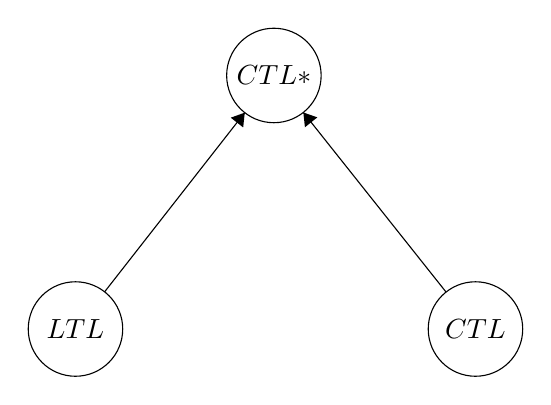
\begin{tikzpicture}[scale=0.2] \tikzstyle{every node}+=[inner sep=0pt] \draw [black] (35.8,-16.1) circle (3); \draw (35.8,-16.1) node {$CTL*$}; \draw [black] (23.2,-32.2) circle (3); \draw (23.2,-32.2) node {$LTL$}; \draw [black] (48.6,-32.2) circle (3); \draw (48.6,-32.2) node {$CTL$}; \draw [black] (25.05,-29.84) -- (33.95,-18.46); \fill [black] (33.95,-18.46) -- (33.06,-18.78) -- (33.85,-19.4); \draw [black] (46.73,-29.85) -- (37.67,-18.45); \fill [black] (37.67,-18.45) -- (37.77,-19.39) -- (38.56,-18.76); \end{tikzpicture} \end{center}

La semantica di queste logiche è basata sulle strutture di Kripke,
ossia 

$\mu=(S,\, I,\,\tau\subseteq S\times S,\, L:\, S\longrightarrow2^{\phi},\, F)$

dove:
\begin{itemize}
\item S è l'insieme degli stati
\item $I\subseteq S$ è l'insieme degli stati iniziali
\item $\tau$ è una relazione tra gli stati totale a sinistra, ossia: $\forall s\in S\,\exists s'\in S\,:\,(s,\, s')\in\tau$
che significa che esistono sempre percorsi di lunghezza infinita.
\item L è la funzione di labelling, che associa ad ogni stato un insieme
di lettere proposizionali, quelle vere nello stato
\item F è l'insieme di stati finali, ovvero l'insieme di stati per cui una
sequenza accettata passa infinitamente spesso
\end{itemize}

\subsection{Grammatica di LTL}

La sintassi di LTL è la più semplice:

una formula ben formata è generata dalla seguente grammatica:

$\varphi\rightarrow P|\neg\varphi|\varphi\wedge\varphi|\varphi\vee\varphi|\varphi\implies\varphi|\varphi\iff\varphi|\next{\varphi}|\eventually{\varphi}|\globally{\varphi}|\until{\varphi}{\varphi}|\release{\varphi}{\varphi}$


\subsection{Grammatica di CTL}

la grammatica di CTL è più complessa, e contiene anche i quantificatori
di cammino, che sono degli operatori che esprimono la verità di una
formula su almeno uno o tutti i cammini, e sono l'operatore E e A
rispettivamente.

i quantificatori di cammino sono vincolati a delle sottoformule specifiche
e non possono essere usati liberamente.

una formula ben formata è generata dalla seguente grammatica:

$\varphi\rightarrow P|\neg\varphi|\varphi\wedge\varphi|\varphi\vee\varphi|\varphi\implies\varphi|\varphi\iff\varphi$

$\varphi\rightarrow A\next{\varphi}|E\next{\varphi}|A\eventually{\varphi}|E\eventually{\varphi}|A\globally{\varphi}|E\globally{\varphi}|A(\until{\varphi}{\varphi})|E(\until{\varphi}{\varphi})|A(\release{\varphi}{\varphi})|E(\release{\varphi}{\varphi})$


\subsection{Grammatica di CTL{*}}

La logica CTL{*} è la logica più complessa e espressiva delle tre.
La sua grammatica è quindi molto più complessa, e si descrive separando
le formule di stato da quelle di cammino:

Sono formule di stato:

$\phi\rightarrow P|\neg\phi|\phi\wedge\phi|\phi\vee\phi|\phi\implies\phi|\phi\iff\phi|A\phi|E\phi$

Sono formule di cammino:

$\varphi\rightarrow\phi|\neg\varphi|\varphi\wedge\varphi|\varphi\vee\varphi|\varphi\implies\varphi|\varphi\iff\varphi|\next{\varphi}|\eventually{\varphi}|\globally{\varphi}|\until{\varphi}{\varphi}|\release{\varphi}{\varphi}$

Le formule di cammino sono formule ben formate (e quindi, anche quelle
di stato).


\subsection{Semantica di CTL{*}}

Per descrivere la semantica di CTL{*} fissiamo una notazione:

sia $\pi$ un cammino $\pi=s_{0},\, s_{1},\, s_{2},\,...$

mentre sia $\pi^{i}$ il suffisso $s_{i},\, s_{i+1},\,...$

$\pi\in s^{\omega}$, ossia appartiene all'insieme delle stringhe
infinite. Si ricordi che:

$s^{\infty}=s^{*}\cup\, s^{\omega}$

La semantica delle formule di stato è definita come:

$\vera{\mu,\pi^{i}}P\iff P\in L(s_{i})$

$\vera{\mu,\pi^{i}}{\neg\phi}\iff\nonvera{\mu,\,\pi^{i}}{\phi}$

$\vera{\mu,\pi^{i}}{\phi\wedge\psi}\iff\vera{\mu,\pi^{i}}{\phi}\,\wedge\,\vera{\mu,\pi^{i}}{\psi}$

$\vera{\mu,\pi^{i}}{\phi\vee\psi}\iff\vera{\mu,\pi^{i}}{\phi}\,\vee\,\vera{\mu,\pi^{i}}{\psi}$

$\vera{\mu,\pi^{i}}{\phi\implies\psi}\iff\nonvera{\mu,\,\pi^{i}}{\phi}\,\vee\,\vera{\mu,\pi^{i}}{\psi}$

$\vera{\mu,\pi^{i}}{(\phi\iff\psi)}\iff(\vera{\mu,\pi^{i}}{\phi}\,\vee\,\vera{\mu,\pi^{i}}{\psi})\vee(\nonvera{\mu,\,\pi^{i}}{\phi}\wedge\nonvera{\mu,\,\pi^{i}}{\psi})$

$\vera{\mu,\pi^{i}}{A\phi}\iff\forall\overline{\pi}\,((\overline{\pi}=s_{i},\,...)\implies(\vera{\mu,\,\overline{\pi}}{\phi))}$

$\vera{\mu,\pi^{i}}{A\phi}\iff\exists\overline{\pi}\,((\overline{\pi}=s_{i},\,...)\implies(\vera{\mu,\,\overline{\pi}}{\phi))}$

La semantica delle formule di cammino è la seguente:

$\vera{\mu,\pi^{i}}{\next{\varphi}}\iff\vera{\mu,\pi^{i+1}}{\varphi}$

$\vera{\mu,\pi^{i}}{\eventually{\varphi}}\iff\exists j\geq i\,:\,\vera{\mu,\pi^{j}}{\varphi}$

$\vera{\mu,\pi^{i}}{\globally{\varphi}}\iff\forall j\geq i\,:\,\vera{\mu,\pi^{j}}{\varphi}$

$\vera{\mu,\pi^{i}}{\until{\varphi}{\psi}}\iff\exists j\geq i\,:\,\vera{\mu,\pi^{j}}{\varphi\,\wedge\,\forall k\,:\, i<k<j}\,\vera{\mu,\,\pi^{k}}{\psi}$

$\vera{\mu,\pi^{i}}{\until{\varphi}{\psi}}\iff\exists j\geq i\,:\,\vera{\mu,\pi^{j}}{\varphi\,\wedge\,\forall k\,:\, i<k<j}\,\vera{\mu,\,\pi^{k}}{\psi}$
<\textcompwordmark{}<sbagliati gli ultimi due, controllare>\textcompwordmark{}>


\section{Model Checking}


\subsection{Definizione}

Il model checking si occupa di risolvere il seguente problema: 

Data una formula $\varphi$ e una struttura di Kripke $\mu$, dire
se $\vera{\mu}{\phi}$ per ogni cammino su $\mu$, ossia:

$\vera{\mu,\,\pi^{0}}{A\varphi}$

In caso contrario esibire un cammino $\pi$ tale che $\nonvera{\mu,\,\pi}{\phi}$\\
\\
Solitamente si verificano 3 tipi di proprietà:
\begin{itemize}
\item Safety: ``non succede mai nulla di grave'' ($\globally{\neg\varphi}$)
\item Liveness: ``prima o poi avviene un evento desiderato'' ($\eventually{\varphi}$)
\item Fairness: ``un evento desiderato avviene infinitamente spesso''
($\globally{\eventually{\varphi}}$)
\end{itemize}
Esistono sostanzialmente due tipologie di tecniche di model checking:
\begin{itemize}
\item Simboliche: basate su tableaux, deduzione formale e SMT solver
\item Operazionali: Basate sulla manipolazione di automi a stati finiti
\end{itemize}

\subsection{Model Checking operazionale}

Il model checking operazionale si basa sulla manipolazione di particolari
automi, detti automi di Büchi.

L'algoritmo alla base è il seguente:
\begin{enumerate}
\item Rappresento il modello $\mu$ con un automa di Büchi $A_{\mu}$
\item per verificare la proprietà $\varphi$, traduco la sua negazione in
un automa di Büchi $A_{\neg\varphi}$
\item Costruisco l'automa prodotto che riconosce il linguaggio intersezione
tra $L(A_{\mu})$ e $L(A_{\neg\varphi})$
\item Controllo se $L(A_{\mu}\times\, A_{\neg\varphi})=\emptyset$, in caso
affermativo la proprietà è verificata.
\end{enumerate}

\subsection{Automi di Büchi}

Gli automi di Büchi sono automi a stati finiti nondeterministici,
che riconoscono linguaggi infiniti, e dove gli stati ``finali''
sono stati di ripetizione, ovvero stati che vengono raggiunti infinite
volte durante il riconoscimento della stringa appartenente al linguaggio.

Gli automi di Büchi godono delle seguenti propietà:

Siano A, B automi di Büchi, allora esiste un automa che riconosce:
\begin{itemize}
\item $L(A)\cup L(B)$
\item $L(A)\cap L(B)$
\item $L(A)^{c}$
\item $L(A)L(B)$ se A è un automa a stati finiti classico
\end{itemize}

\subsection{Da formule di LTL ad automi di Büchi}

Esiste un algoritmo per tradurre una formula di LTL in un automa di
Büchi. Lo stesso algoritmo si può estendere, con le dovute accortezze
e prestando attenzione ai sottocasi, alle formule di CTL e CTL{*}.

Sia $\varphi$ la formula e siano $P_{1},\,...,\, P_{n}$ le lettere
predicative di $\varphi$

Si può trovare un automa di Büchi $A_{\varphi}=(S,\, I,\,\tau,\, L,\, F)$
con $L:\, S\longrightarrow2^{\{P_{1},\,...,\, P_{n}\}}$tale che,
se $\pi$ è un path che corrisponde ad una parola $\omega\in L(A_{\varphi})$,
allora $\vera{(S,\,\tau,\, L),\,\pi}{\varphi}$

l'algoritmo è il seguente:
\begin{enumerate}
\item Porto la formula $\varphi$ in forma negata normale
\item elimino i globally ($\mathcal{G}$)
\item Costruisco l'automa locale $A_{L}$
\item altro che non abbiamo fatto
\end{enumerate}

\subsubsection{Forma negata normale }

Portare una formula in forma negata normale, consiste nel rendere
una formula più ``semplice'', cioè in modo che contenga ``pochi''
connettivi e operatori modali diversi, avendo cura di portare le negazioni
davanti alle lettere proposizionali.

Per farlo utilizzo le seguenti regole:

I) Le relazioni tra gli operatori modali 
\begin{itemize}
\item $\neg\globally{a\equiv\eventually{\neg a}}$
\item $\neg\eventually a\equiv\globally{\neg a}$
\item $\neg(\until a{b)}\equiv(\release{\neg a}{\neg b})$
\item $\neg(\release ab)\equiv(\until{\neg a}{\neg b})$
\end{itemize}
II) Le formule di De Morgan
\begin{itemize}
\item $\neg(a\wedge b)\equiv(\neg a)\vee(\neg b)$
\item $\neg(a\vee b)\equiv(\neg a)\wedge(\neg b)$
\end{itemize}
La formula così trovata si dice in forma negata normale.

Si può a questo punto eliminare anche l'operatore globally, ricordando
la seguante relazione:
\begin{itemize}
\item $\globally a\equiv\release{\bot}a$
\end{itemize}

\subsubsection{Costruzione dell'automa locale}

L'automa locale è un automa che riconosce sequenze di esecuzione che
verificano la proprietà $\varphi$

l'algoritmo si articola in due passi:
\begin{enumerate}
\item Chiusura della formila $\varphi$: $cl(\varphi)$

\begin{itemize}
\item $\varphi\in cl(\varphi)$
\item $\psi\in cl(\varphi)\implies\neg\psi\in cl(\varphi)$
\item $\psi\wedge\theta\in cl(\varphi)\implies\psi,\theta\in cl(\varphi)$
\item $\psi\vee\theta\in cl(\varphi)\implies\psi,\theta\in cl(\varphi)$
\item $\next{\psi}\in cl(\varphi)\implies\neg\psi\in cl(\varphi)$
\item $\eventually{\psi}\in cl(\varphi)\implies\neg\psi\in cl(\varphi)$
\item $\until{\psi}{\theta}\in cl(\varphi)\implies\psi,\theta\in cl(\varphi)$
\item $\release{\psi}{\theta}\in cl(\varphi)\implies\psi,\theta\in cl(\varphi)$
\end{itemize}
\item Automa locale $A_{L}=(\Sigma,\, S_{L},\, I_{L},\,\tau_{L},\, F_{L})$

\begin{itemize}
\item $\Sigma=2^{cl(\varphi)}$ ovvero $\Sigma\subseteq\mathcal{P}(cl(\varphi))$
\item $S_{L}$ formato da tutti gli elementi di $\Sigma$ consistenti ovvero
$\psi\in S_{L}\iff\neg\psi\notin S_{L}$
\item $I_{L}=\{s\in S_{L}\,|\,\varphi\in s\}$
\item $F_{L}=S_{L}$ (ossia tutti gli stati sono finali)
\item $\tau_{L}$ tale che: siano $s,s'\in S_{L}$, $a\in\Sigma$ allora
$(s,\, a,\, s')\in\tau_{L}$ se e solo se:

\begin{enumerate}
\item $a=s$
\item $\next{\psi\in s\iff\psi\in s'}$
\item $\eventually{\psi\in s\iff\psi\in s'\,\vee\,\eventually{\psi\in s'}}$
(infatti vale $\eventually{\psi}\equiv\next{\psi}\vee\next{\eventually{\psi}}$)
\item $\until{\psi}{\theta}\in s\iff\theta\in s'\,\vee\,(\psi\in s\,\wedge\,\until{\psi}{\theta\in s')}$
(infatti vale $\until{\psi}{\theta}\equiv\next{\theta\vee(\psi\wedge\next{(\until{\psi}{\theta}}))}$)
\item $\release{\psi}{\theta}\in s\iff\psi\wedge\theta\in s\,\vee\,(\theta\in s\,\wedge\,\release{\psi}{\theta\in s')}$
\end{enumerate}
\end{itemize}
\end{enumerate}
Una volta costruito l'automa in queosto modo, si deve minimizzare.
L'automa minimo è l'automa locale di $\varphi$


\subsubsection*{Esempio}

<\textcompwordmark{}<MANCA>\textcompwordmark{}>
